
Bio-locomotion using high Reynolds number (Re) unsteady fluid dynamics is an active area of research.
The ability of many birds \cite{warrick2005aerodynamics}, mammals \cite{fish2006passive,muijres2008leading}, insects \cite{ellington1996leading,srygley2002unconventional,sane2003aerodynamics,ellington1999novel,wang2005dissecting}, fish \cite{fish2006passive,triantafyllou2000hydrodynamics} (depicted in Figure \ref{fig:Insects}) to control the unsteady flow around them currently appears to be outside the range of robotic mimics.
Effective manipulation and control of unsteady effects at high Reynolds numbers are considered to underlie the superior performance of these organisms.
As the robotics community pushes the limits on engineering, it is useful to know the fundamental performance limits under various fluid-structure interaction setting, e.g. maximum propulsive power of a flexible fin \cite{tokic2012optimal,van2013optimal,milano2005uncovering,eloy2011optimisation}, or the maximum lift possible from a periodically flapping wing \cite{kawamura2008clapping,karpelson2010energetics,wood2008first}.
The set of beneficial unsteady effects is small and hence, has proved difficult to find \cite{pesavento2009flapping}.
The challenge is to develop a reasonable strategy for scanning the large space of all possible motions and deformations of the body to determine the beneficial set.
Optimization and control theory, with calculus of variations at its foundation \cite{lions1971optimal}, provides a framework fro tackling this complexity.
Steady progress on a control theoretic framework applied to steady and unsteady fluid dynamics has resulted in significant advances since the late 1980s \cite{jameson1988aerodynamic,jameson1998optimum,bewley2000general,kim2007linear,wang2009minimal,yu2013high,culbreth2013high}.
In a nutshell, the strategy is to couple methods of solving the governing Navier-Stokes equations with adjoint-based gradient calculations to facilitate optimization and control.
For example to find the maximum lift possible from the unsteady stroke of a wing, one can use gradient descent algorithms.
However, the presence of nonlinearities and multiple scales in the fluid dynamics impedes rapid computation of the flow.

\begin{figure}
\begin{center}
\begin{tabular}[t]{ccc}
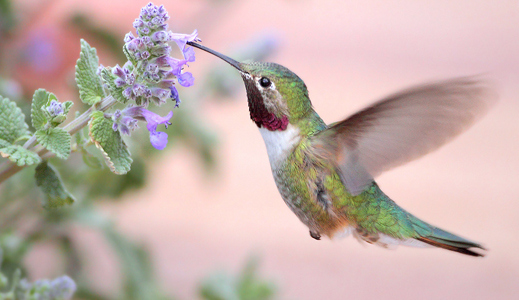
\includegraphics[height=3cm]{./Figures/intro/hummingbird.jpg} & 
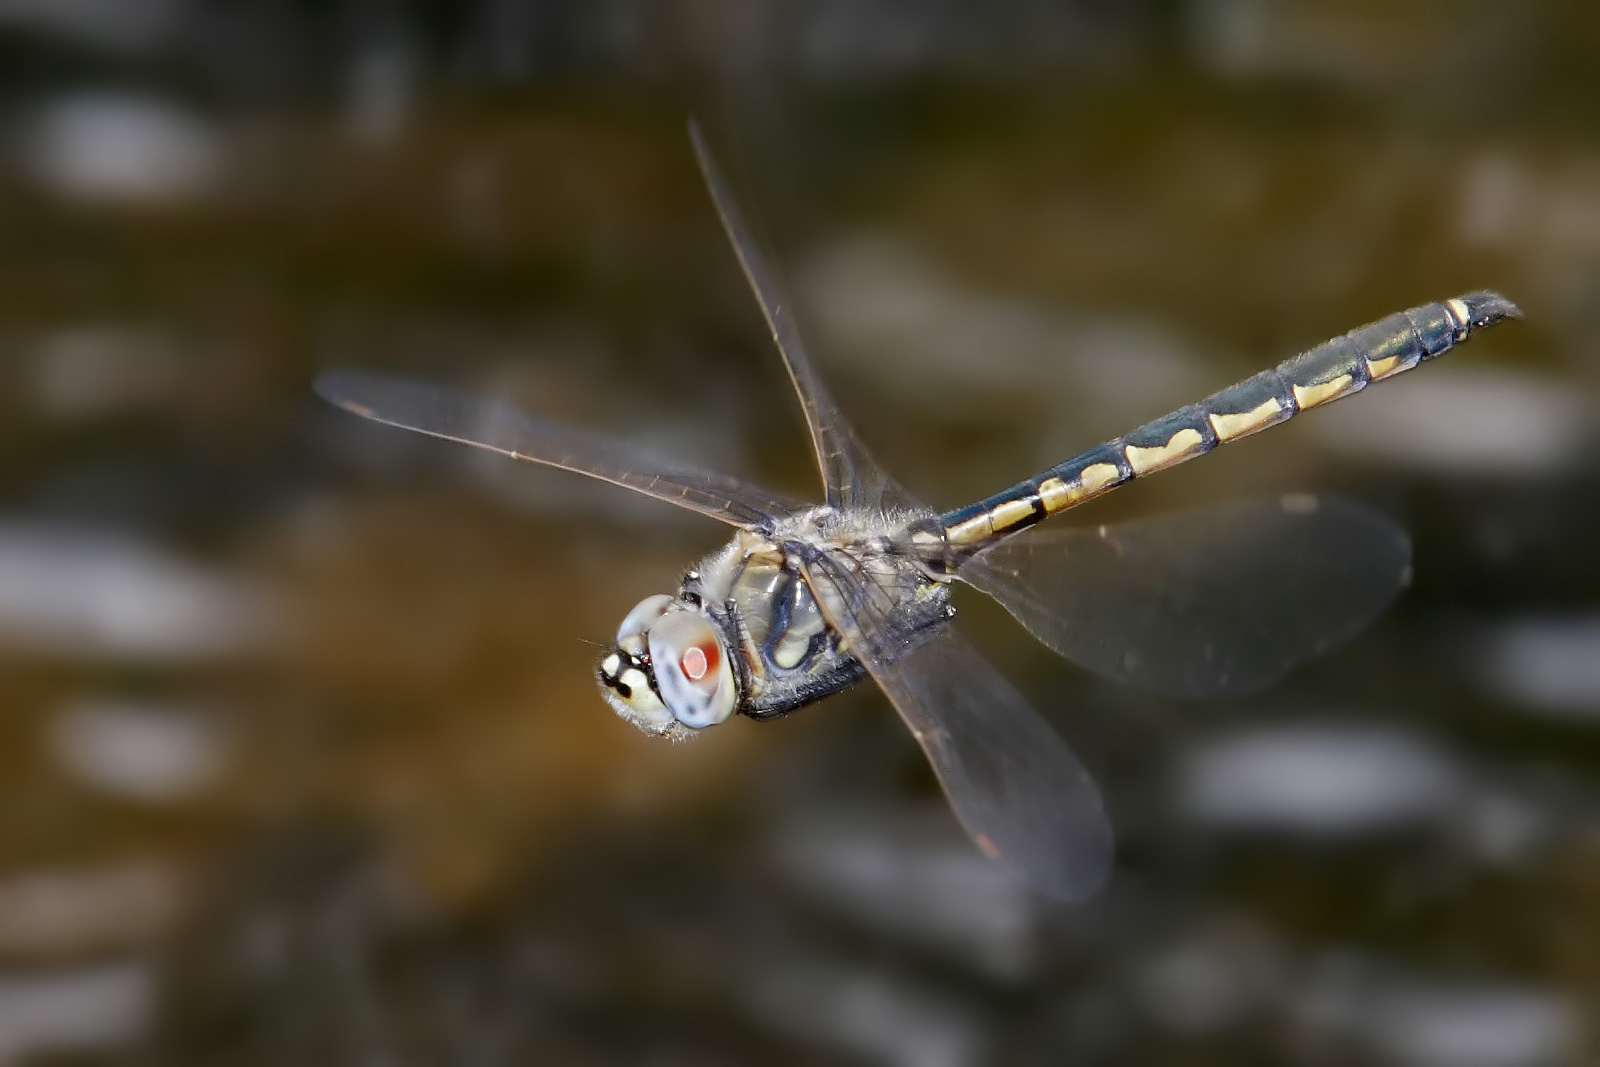
\includegraphics[height=3cm]{./Figures/intro/insect.jpg} & 
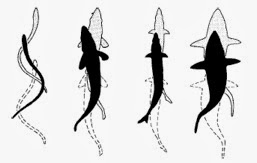
\includegraphics[height=3cm]{./Figures/intro/fish.jpg} \\
(a) &
(b) &
(c)
\end{tabular}
\end{center}
\caption[Locomotion of birds, insects and fish using unsteady fluid dynamics]{Propulsive strokes of (a) birds and (b) insects, and (c) fish impart them with capabilities difficult to reproduce technologically.}
\label{fig:Insects}
\end{figure}

\section{Description of the problem}

Separated flows, in which the fluid fails to smoothly follow the solid surface, in contrast with attached flows, are generally more complex and more challenging to measure or predict.
It was shown by Prandtl that, for the same conditions, the viscous equations and the inviscid equations can have very different solutions even if viscosity is extremely weak, precisely because the viscous flow might separate while the inviscid flow does not.
Flows at high Reynolds numbers (low viscosity) are thus very sensitive and, by and large, we only have a qualitative and sometimes simplistic knowledge of their behavior.

In most designs, separation is undesirable since it results in inefficient operation, with high drag or loss of pressure, or even it leads to a dangerous situation like stall.
However many devices, like wings or diffusers, often operate on the verge of separation.
In other cases separation is present in the design conditions, where it is undesirable but unavoidable, like an aircraft tails or cars, or a normal feature of the flow, like on a three dimensional wing.

A relevant example is the flow around the retreating blade of a helicopter in translation.
The blade experiences large and rapid changes of incidence and velocity, sufficient to cause stall with strong unsteady effects.
The blade may even move with the trailing edge forward for part of the cycle, which always causes separation.
The dynamics stability of the system strongly depends on the aerodynamic loads, especially the pitching moment, and these exhibit very significant non-linear and hysteric effects.
Figure ?? illustrates how much the loads can differ during dynamic stall from static loads at the same incidence.
Accurately predicting dynamic stall would thus be very useful, and should be possible in the near future (at least for two-dimensional flow), thanks to improvements in numerical methods and computers.

Experimental results demonstrate the strong sensitivity of separated flows to details of body geometry, for instance surface roughness, and of course to the Reynolds number.
The best known example is the circular cylinder: this flow still exhibits dramatic changes at Reynolds numbers of one million (Fig. 2 and 3).
Wind tunnel tests are less reliable when fine viscous effects are involved than when the compressibility effects dominate, because the Reynolds number depends on model size, while the Mach number does not, and because separation is influenced by wind-tunnel turbulence.
Analysis alone has not been able to produce many results, mainly because separated flows can rarely be treated as slightly perturbed from a known exact solution: they are not very accessible to small disturbance theories.
Free streamline theory made use of the observation that, in many cases, drag depends mostly on the forebody shape (upstream of the separation point) and very little on the part of the body which is inside the wake.
Pressure also appears to be almost constant in that region.
The idea developed was to treat the wake as a "dead-water" region and to assume a constant pressure in that region; in general the value of the base pressure is determined empirically.
This theory did produce some good results, but a method that ignores the unsteady character of the flow cannot be expected to be very accurate; it relies very much on empiricism.
Thus there is an existing need for the development of numerical methods capable of solving either the full Navier-Stokes equations or a high level approximation to them without relying on much empirical input.
Once these methods have reached an acceptable level of accuracy, they are expected to be much faster and less expensive than large scale wind tunnel tests, and amy be more accurate if they are carefully validated against fight tests.

Whereas accurate and practical numerical methods are available to compute attached flows, similar methods do not exist for separated flows, which are vortical.
The slowly-varying, attached, irrotational flows are very amenable to finite difference or finite element methods, and to an Eulerian formulation.
Some of these methods can also treat separated flows, but obtaining accurate results becomes extremely costly at moderate or high Reynolds numbers.
One alternative is the Lagrangian "Vortex Method".
This method provides a description which is better adapted to high-Reynolds number, vorticity-dominated, unsteady flows, and should result in a greater accuracy for a given level of computing resources.

The first objective of this work was to study the capabilities of the Vortex Method, review its inherent strengths and weakness, especially in the context of two-dimensional separated flows, and remedy some of the weakness.
The other objective was to develop a reliable and accurate computer program, based on the Vortex Method, for the simulation of a general class of separated flows.
This program has been validated by systematic comparison with known results, and is beginning to be used as an active research tool to investigate some candidate designed, in parallel with wind tunnel tests.

The flows to be considered are viscous flows past two-dimensional solid bodies in a uniform stream.
Only incompressible flows are considered.
The incompressibility limitation is associated with the Vortex Method.
The two-dimensional restriction is not, but simulating two-dimensional flows is a first step and reflects the "state of the art".
(The extension to three dimensions would not be straightforward, but it is certainly possible.)
We consider here one or more bodies and they may be in non-uniform motion.
Even if the motion is uniform, the flow is likely to be unsteady with a possible periodic character.
Frequently separation of the boundary layer will occur as a result of the body being bluff or at high angles of attack.
Large vortical structures will appear and form a wake having a turbulent character, and these structures will strongly influence the loads on the body.
Their subsequent decay in the wake far downstream is of less interest because of their small influence on the loads.
Again, typical examples are the flow past a circular cylinder, and the static or dynamic stall of an airfoil.


\section{Related investigations}

Numerically solving the governing Navier-Stokes equations using primitive variables is prohibitively expensive from the perspective of flow optimization and control.
A simple back-of-the-envelope estimate of the computational effort for solving the flow corresponding to a Reynolds numbers of $10^4$, shown in table 1, highlights this issue.
The primary expense arises from resolving the boundary layer; its thickness dictates the number of grid points to be used for spatial discretization, and the time step through the CFL condition.
On modern desktop computers one flow solution in 2D takes at least hours, and in 3D takes at least days. (The computational effort shown in table \ref{table:DNS} is grossly underestimated; flow past stationary, moving and flexible bodies at $Re = 10 - 10^3$ takes a few CPU-days in 2D \cite{mittal2005immersed}, and CPU-weeks in 3D \cite{pesavento2009flapping,mittal2005immersed}, and very little data is available for larger $Re$.)
Calculating the adjoint variables and implementing a gradient based optimization algorithm \cite{wang2009minimal} increases the computational time to at least months for 2D problems (yeas for 3D).
Methods like Large Eddy Simulations model sub-grid scale eddies, but still have to resolve the boundary layer to accurately predict the shed vorticity, and hence are not exempt from this estimate.
Parallel computing on a cluster of processors can reduce the 2D computational time to few days and today's top 5 supercomputers may be able to reduce the computational time for 3D to several hours, if the algorithms are effectively parallelized, but it is uncertain how data dependencies can be addressed for parallelization.
In conclusion, optimization, state estimation, and control are still out of range of computation fluid dynamics.

\begin{table}[h] 
\small
\begin{tabular}{| p{3.5cm} | l l | l l |}
\hline
                                                                      &       2D scaling                                         &      Estimate                &           3D scaling                                   &             Estimate              \\
\hline
Reynolds number                                      &      $Re = Ua/\nu$                                    &      $10^4$                &            $Re = Ua/\nu$                             &            $10^4$                \\
Boundary layer thickness                        &      $\delta=aRe^{-1/2}$                          &      $10^{-2}a$           &            $\delta=aRe^{-1/2}$                   &           $10^{-2}a$          \\
Grid spacing                                               &     $h = \delta/10$                                    &      $10^{-3}a$           &            $ h = \delta/10$                           &            $10^{-3}a$          \\
Number of grid points                               &     $N_g = a^2/h^2$                                &      $10^6$                 &            $N_g = a^3/h^3$                        &            $10^9$                 \\
Time step limit                                            &     $\Delta t = h/U$                                   &      $10^{-3}a/U$       &            $\Delta t = h/U$                           &            $10^{-3}a/U$       \\
Number of time steps                                &     $N_t = 10a/U\Delta t$                       &       $10^4$                 &            $N_t = 10a/U\Delta t$                &            $10^4$                 \\
Flops per time step                                    &     $N_s = 10^3N_g\log N_g$              &      $10^{10}$             &            $N_s = 10^3N_g\log N_g$       &           $10^{10}$            \\
Flops per solution                                      &     $N_{sol} = N_s N_t $                        &       $10^{14}$            &             $N_{sol} = N_s N_t $                 &           $10^{16}$            \\
Flops per adjoint                                        &     $N_{adj} = N_{sol} \log N_t $          &       $10^{14}$            &             $N_{sol} = N_s N_t $                 &           $10^{16}$             \\
Number of iterations for optimization     &     $N_{iter}$                                            &       $20$                     &             $N_{iter} $                                    &           $20$                      \\
Total flops for optimization                       &     $N_{adj} N_{iter}$                             &       $10^{16}$            &             $N_{adj} N_{iter} $                     &           $10^{18}$             \\
Desktop speed                                           &     $R$ (in flops/sec)                              &       $10^{10}$            &              $R$ (in flops/sec)                       &          $10^{10}$              \\
Wall time per solution                               &     $t_w = N_{sol}/R$                              &       $10^4$ sec         &              $t_w = N_{sol}/R$                      &          $10^6$ sec            \\
Wall time per adjoint                                 &     $t_{adj} = N_{adj}/R$                       &        $10^5$ sec         &              $t_{adj} = N_{adj}/R$                 &          $10^7$ sec            \\
Total wall time for optimization               &     $t_{total} = N_{iter} t_{adj}$             &        $O$(months)      &              $t_{total} = N_{iter} t_{adj}$      &          $O$(years)             \\
\hline
\end{tabular}
\caption[An estimate of computational complexity of direct numerical simulation]{An order-of-magnitude estimate of the computational complexity and expected computational wall time for the execution of stroke optimization for flow of characteristic speed $U$ past a body of characteristic size $a$ at a Reynolds number of $10^4$. The various prefactors governing the accuracy of the solution are chosen here to reflect the best estimates from literature, but err on the side of under-estimation. Real computational time experienced by researchers is higher by up to two orders of magnitude.}
\label{table:DNS}
\end{table}


An hierarchy of reduced order models of fluid flow provide an alternative to avoid the computational effort for the solution of Navier-Stokes equations, at the expense of reduced (or sometimes uncertain) accuracy.
All these models identify that viscous effects in the flow may be neglected except for the process of vorticity shedding from the body.
The simplest of these models \cite{tanabe1994behavior,mahadevan1996tumbling,belmonte1998flutter,mahadevan1999tumbling,pesavento2004falling,andersen2005unsteady} apply to rigid wings.
They assume the flow around the wings to be qui-steady and model the fluid dynamic force on them in terms of the instantaneous orientation, velocity and acceleration of the wing.
Versions of such models that incorporate unsteadiness \cite{hansen2004beddoes,brunton2013empirical} are also available.
The assumptions underlying these models make them unsuitable for large amplitude unsteady motion, where the flow can separate from multiple points on the body.

Models in the next level of hierarchy also only apply to bodies with sharp edges, but model vorticity transport according to inviscid dynamics \cite{pedley1999large,jones2005falling,shukla2007inviscid,singh2008hydrodynamics,alben2009simulating,michelin2009unsteady,michelin2010falling,sheng2012simulating}.
These models assume that vorticity is shed only from the sharp edges of the body and then evolves into a vortex sheet.
The rate of the vorticity shed is chosen so as to eliminate a singularity of the flow at these sharp edges - the celebrated Kutta condition from aerodynamics.
The shed vortex sheet is usually represented by an array of discrete point vortices obeying inviscid vortex dynamics or a single tightly rolled-up point vortex (governed by the Brown-Michael vortex dynamics).
These methods are also very efficient.
However, they do not allow for the possibility of separation at any point other than one of the sharp edges on the body.
As a result, they cannot be used to model vorticity shed from a smooth body (e.g. an elliptical wing).
Moreover, in practice, vorticity is not always shed from the leading edge of a wing.
These methods cannot a priori predict the edges at which the flow separates.
Because the optimal flows are suspected to correspond to a precise control of the instance vorticity shedding switches on or off from one of the edges, or of shedding from another point on the surface of body, these models appear to mis-represent or eliminate the effects underlying the enhanced unsteady performance.

The most accurate and computationally intensive methods in the hierarchy account for the vorticity in the boundary layer as vortex sheets of variable strength at or near the surface of the body.
The vortex sheets are represented as arrays of point of blob vortices and function to enforce the no-slip condition \cite{shukla2007inviscid,chorin1978vortex,leonard1980vortex,sethian1988validation,anderson1989vorticity,koumoutsakos1994boundary,summers1996numerical,eldredge2002vortex}.
These vortices transport away from the boundary by advection and diffusion, and leave the boundary layer where the flow separates, thus accurately modeling vorticity shedding.
The drawback of this method is that accurate description of flow requires computational effort comparable to direct solution of Navier-Stokes equations.
It is so because the distance between the point or blob vortices should be comparable to a fraction of the boundary layer thickness, and play a role analogous to grid spacing in direct solution of Navier-Stokes equations.
These methods are not reduced order models in the strict sense, because they apply for all $Re$ and do not take advantage of the large $Re$ of the flow.
